\documentclass{article}
\usepackage{graphicx} % Required for inserting images
\usepackage{amsmath}
\usepackage[margin = 1in]{geometry}
\title{The Effect of Linear Transformations of Periodic Functions on the Fourier Series Representation}
\author{Shruti Shrirang Karandikar}
\date{June 2025}
%\geometry{vmargin = (1in), hmargin = (1in, 1in)}
\begin{document}

\maketitle

\section{Introduction}

Fourier series are powerful mathematical tools that allow us to represent periodic functions as infinite sums of sine and cosine terms. Named after the French mathematician Jean-Baptiste Joseph Fourier (1768-1830), these series have profound applications in various fields including signal processing, physics, engineering, and data analysis.\\

At their core, Fourier series express a periodic function as a weighted sum of sinusoids (sine and cosine functions) of different frequencies. Each sinusoid contributes to the overall shape of the function, with the weights (coefficients) determining how much each frequency component contributes to the final representation. This decomposition reveals the frequency content of a signal, providing insights into its fundamental characteristics.\\

In this paper, we examine what happens to the Fourier representation when a function is transformed. These transformations include horizontal shifts (time or space delays), vertical shifts (amplitude offsets), stretching, and compression of functions. When we apply these operations to a function in the time or space domain, its Fourier representation changes in specific and predictable ways.\\

The shifting and scaling properties of Fourier series demonstrate elegant mathematical relationships. For instance, a horizontal shift in the time domain corresponds to a phase shift in the frequency domain, while stretching a function compresses its frequency representation and vice versa.\\

This paper aims to provide an accessible introduction to Fourier series transformations, focusing on the core concepts and developing an intuition about the impact of the transformations. By understanding how these basic operations affect Fourier representations, we gain powerful insights into signal analysis and processing techniques used across multiple disciplines.\\

\section{General Fourier Series Equations}

The general equations for a Fourier series of a periodic function $f(x)$ with period $2L$ is given by:

\begin{enumerate}
    \item Synthesis Equation
    \begin{equation}
    f(x) = \frac{a_0}{2} + \sum_{n=1}^{\infty} \left[ a_n \cos\left(\frac{nx\pi}{L}\right) + b_n \sin\left(\frac{nx\pi}{L}\right) \right] 
    \end{equation}
Where the coefficients are determined by the following analysis equations:

    \item Analysis Equations
    \begin{eqnarray}
    a_0 =& \frac{1}{L}& \int_{-L}^{L} f(x) \, dx
    \nonumber\\
a_n =& \frac{1}{L}& \int_{-L}^{L} f(x) \cos\left(\frac{nx\pi}{L}\right) \, dx, \quad n \geq 1\label{eqn:Analysis Equations}\\
b_n =& \frac{1}{L}& \int_{-L}^{L} f(x) \sin\left(\frac{nx\pi}{L}\right) \, dx, \quad n \geq 1
\nonumber
    \end{eqnarray}
\end{enumerate}

\section{Square Wave}
\begin{figure}
    \centering
    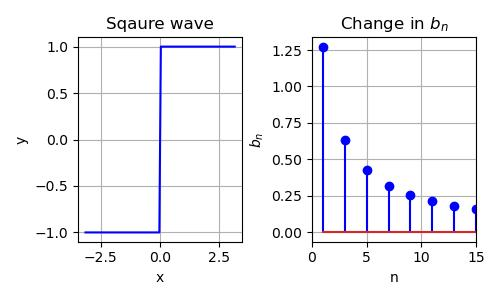
\includegraphics[width=0.8\textwidth]{sqaurewave.jpg}
    \caption{Square Wave}
    \label{fig: Square Wave}
\end{figure}
The standard square wave function with period $2L$ and amplitude $A$ can be defined as:
\begin{equation}
    f(x) = 
\begin{cases} 
-A&     -L < x < 0 \\
~~A&      0 < x < L
\end{cases}
    \end{equation}
When we compute the Fourier coefficients for this square wave, we get:
\begin{eqnarray}
a_0 &=& 0 \nonumber\\
a_n &=& 0 \quad\quad\quad \text{for all } n\\
b_n &=& 
\begin{cases} 
\frac{4A}{n\pi}, & \text{for odd } n \\
0, & \text{for even } n\nonumber
\end{cases}
\end{eqnarray}
Therefore, the Fourier series for the standard square wave becomes: 
\begin{eqnarray}
    f(x) =  \sum_{n=1,3,5,...}^{\infty} \frac{4A}{n\pi} \sin\left(\frac{n\pi x}{L}\right)
\end{eqnarray}\\
For the transformations we will look at a special case:
\begin{equation}
f(x) = 
\begin{cases} 
-1, & -\pi < x < 0 \\
1, & 0 < x < \pi
\end{cases}
\end{equation}
And the Fourier series is:
$$f(x) =  \sum_{n=1,3,5,...}^{\infty} \frac{4}{n\pi} \sin\left(n x\right)$$
These are visualized  in Figure \ref{fig: Square Wave}.


\section{Transformations of Functions}

In this section, we explore how various transformations of a function affect its Fourier series representation. Using the square wave as our example, we'll examine four fundamental transformations: vertical shifting, horizontal shifting, vertical scaling, and horizontal scaling.

\subsection{Vertical Shifting}   
Consider a vertical shift of 1, then the function becomes (as shown in figure \ref{vertical shifting}):
\begin{equation}
g(x) = 
\begin{cases} 
0, & -\pi < x < 0 \\
2, & 0 < x < \pi
\end{cases}
\end{equation}

\begin{figure}[t]
    \centering
    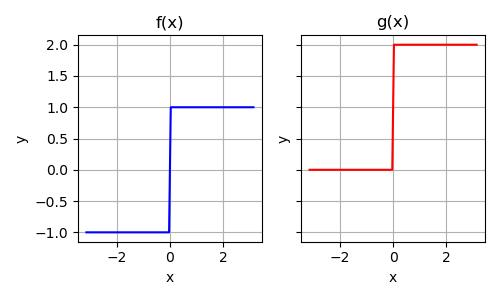
\includegraphics[width=0.8\textwidth]{vertical_shift.jpg}
    \caption{Vertical Shifting}
    \label{vertical shifting}
\end{figure}
Using equation (\ref{eqn:Analysis Equations}), for this square wave, we get:
    \begin{eqnarray}
    a_0 =& 2\nonumber\\
    a_n =& 0\\
    b_n =& \frac{4}{n\pi} \nonumber
    \end{eqnarray}
The Fourier series then becomes:
    \begin{equation}
g(x) = 1 + \sum_{n=1,3,5,...}^{\infty} \frac{4}{n\pi} \sin\left(nx\right)
    \end{equation}
When the square wave alternates between $-1$ and $1$ over the interval $[-\pi, \pi]$, its average value is $0$, meaning there's no "constant component" in the signal - it spends equal time above and below the x-axis.
\vspace{0.2in}

When we vertically shift this square wave upward by $1$ unit (creating a function that alternates between $0$ and $2$), the shape of the wave remains identical - all the rises and falls occur at exactly the same places. The only difference is that the entire wave now hovers higher on the y-axis. In frequency terms:

\begin{enumerate}
\item The DC component $(a_0)$ increases from $0$ to $1$, representing the new average height of the function
\item All other Fourier coefficients remain unchanged because the pattern of variation hasn't changed at all
\end{enumerate}\\

The DC component $(a_0)$ acts like the "baseline" or "center of gravity" of our function. When we vertically shift a function, we are simply adjusting where this baseline sits, without affecting any of the actual oscillatory behavior that's captured by the other Fourier coefficients.

\subsection{Horizontal Shifting}
Consider a horizontal shift of $\pi$, then the function becomes (as shown in \ref{fig: horizontal shift}):
\begin{equation}
g(x) = 
\begin{cases} 
-1, & 0 < x < \pi \\
1, & \pi < x < 2\pi
\end{cases}
\end{equation}\\
\begin{figure}
    \centering
    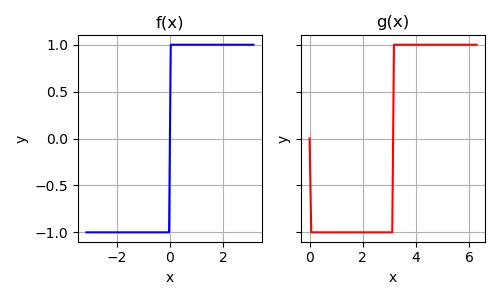
\includegraphics[width=0.8\textwidth]{horizontal_shift.jpg}
    \caption{Horizontal Shifting}
    \label{fig: horizontal shift}
\end{figure}
Using equation (\ref{eqn:Analysis Equations}), for this square wave, we get:
    \begin{eqnarray}
    a_0 =& 0\nonumber\\
    a_n =& 0\\
    b_n =& \frac{-4}{n\pi}\nonumber
    \end{eqnarray}  
The Fourier series then becomes:
\begin{equation}
g(x) = \sum_{n=1,3,5,...}^{\infty} \frac{-4}{n\pi} \sin\left(nx\right)
\end{equation}
When we horizontally shift a square wave, we are essentially moving all its features along the x-axis. This transformation helps us to understand a key property of Fourier series: horizontal shifts correspond to phase changes in the frequency domain.
\vspace{0.2in}

Consider our original square wave that alternates between $-1$ and $1$. When we shift it horizontally, say by $\pi$ units, the function itself looks identical in shape but is now positioned differently along the x-axis.
\vspace{0.2in}

Looking at the Fourier coefficients after this shift, we notice something interesting:

\begin{enumerate}
\item The magnitudes of all coefficients remain unchanged
\item However, the sine coefficients $(b_n)$ change sign
\end{enumerate}\\

This sign change can be understood through the trigonometric identity $\sin(-nx) = \sin(\pi + nx)$. What this tells us is that when the sine coefficients change sign, it's equivalent to adding a phase shift of $\pi$ to each frequency component.
\begin{equation}
g(x) = \sum_{n=1,3,5,...}^{\infty} \frac{4}{n\pi} \sin\left(\pi+nx\right)
\end{equation}

More generally, when we shift a function horizontally by some amount $h$, each frequency component in the Fourier series experiences a phase shift proportional to its frequency. The sine waves don't change their amplitudes - they simply start at different points in their cycles.
\vspace{0.2in}

Think of it like this: if we push a wave pattern sideways, we haven't changed how the wave goes up and down (its amplitude), but we have changed when it goes up and down (its phase).
\vspace{0.2in}

This is why we say a horizontal shift in the time/space domain corresponds to a phase change in the frequency domain. The energy at each frequency stays the same, but the timing information shifts.

\subsection{Vertical Scaling}
\begin{figure}[t]
    \centering
    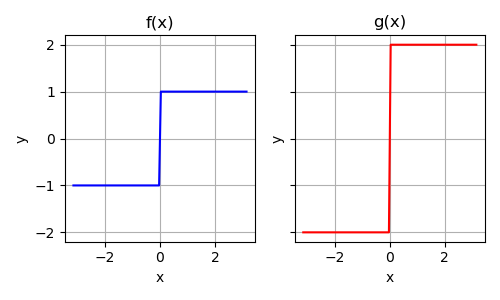
\includegraphics[width=0.8\textwidth]{vertical_scaling.png}
    \caption{Vertical Scaling}
    \label{Vertical Scaling}
\end{figure}
Consider a vertical stretch of 2, then the function becomes (as shown in Figure \ref{Vertical Scaling}): 
\begin{equation}
g(x) = 
\begin{cases} 
-2, & -\pi < x < 0 \\
2, & 0 < x < \pi
\end{cases}
\end{equation}\\
\begin{figure}[h]
    \centering
    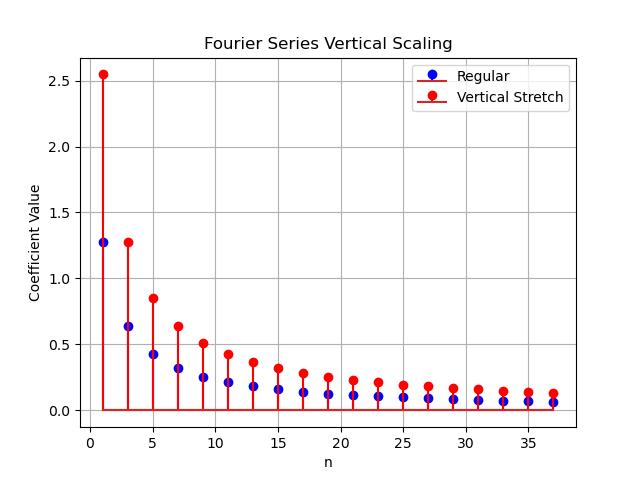
\includegraphics[width=0.8\textwidth]{vertical_stem_stretch.jpg}
    \caption{Change in $b_n$}
    \label{vertical_stem_stretch}
\end{figure}
Using equation (\ref{eqn:Analysis Equations}), for this square wave, we get:
    \begin{eqnarray}
    a_0 =& 0\nonumber\\
    a_n =& 0\\
    b_n =& \frac{8}{n\pi}\nonumber\\
    \end{eqnarray}
The Fourier series then becomes:
    \begin{equation}
g(x) = \sum_{n=1,3,5,...}^{\infty} \frac{8}{n\pi} \sin\left(nx\right)
    \end{equation}
When we vertically scale a function, we're essentially making its excursions from the x-axis more dramatic. For our square wave that originally oscillated between $-1$ and $1$, a vertical scaling by a factor of $2$ creates a new function that oscillates between $-2$ and $2$.
\vspace{0.2in}

Looking at the Fourier coefficients after this transformation, we observe a direct and intuitive relationship:

\begin{enumerate}
\item All Fourier coefficients $(b_n)$ are scaled by exactly the same factor $(2)$
\item The overall shape or "profile" of the frequency spectrum remains unchanged\\
\end{enumerate}
The stem plot (Figure \ref{vertical_stem_stretch}) visually confirms this relationship. Looking at the original square wave's $b_n$ coefficients alongside the scaled version's coefficients, we can see that each frequency component has been amplified by the same factor of $2$. The taller stems in the scaled function's plot are exactly twice as high as the corresponding stems in the original function's plot.
\vspace{0.2in}

This makes intuitive sense if we think about what the Fourier coefficients represent. Each coefficient tells us "how much" of a particular frequency component is present in our function. When we amplify the function itself, we're proportionally amplifying all of its constituent components.
\vspace{0.2in}

The stem plot elegantly demonstrates this preservation of relative strengths between frequency components. The characteristic "decreasing staircase" pattern of the square wave's Fourier coefficients (where $b_n = 0$ for even $n$, and $b_n = \frac{4}{n\pi})$ for odd $n$) maintains its distinctive shape, just scaled to a larger magnitude.\\

This relationship highlights an important property of Fourier series: linear scaling in the time/space domain corresponds directly to linear scaling in the frequency domain, preserving the relative "fingerprint" of the function's frequency content.  

\subsection{Horizontal Scaling}
Consider a horizontal scale of 2, then the function becomes (as shown in Figure \ref{Horizontal_Scaling}) :
\begin{equation}
g(x) = 
\begin{cases} 
-1, & -2\pi < x < 0 \\
1, & 0 < x < 2\pi
\end{cases}
\end{equation}\\
\begin{figure}[t]
    \centering
    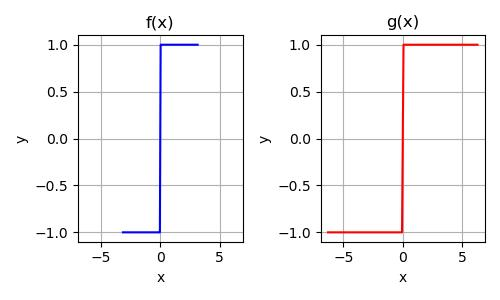
\includegraphics[width=0.8\textwidth]{horizontal_scaling.jpg}
    \caption{Horizontal Scaling}
    \label{Horizontal_Scaling}
\end{figure}
\begin{figure}[h]
    \centering
    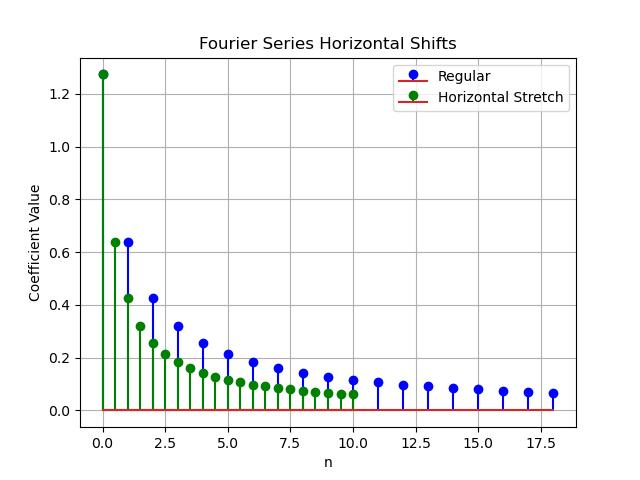
\includegraphics[width=\textwidth]{horizontal_stem_stretch.jpg}
    \caption{Change in $b_n$}
    \label{fig:horizontal_stem_stretch}
\end{figure}
Using equation (\ref{eqn:Analysis Equations}), for this square wave, we get:
    \begin{eqnarray}
    a_0 =& 0\nonumber\\
    a_n =& 0\\
    b_n =& \frac{4}{\pi}\nonumber\\
    \end{eqnarray}
The Fourier series then becomes:
\begin{equation}
g(x) = \sum_{n=1,3,5,...}^{\infty} \frac{4}{n\pi} \sin\left(\frac{nx}{2}\right)
\end{equation}
When we horizontally scale our square wave, stretching it from the interval $[-\pi, \pi]$ to $[-2\pi, 2\pi]$, we're essentially "spreading out" the function along the x-axis. This transformation provides fascinating insights into how the frequency content adapts when a signal is stretched or compressed in time/space.
\vspace{0.2in}

Looking at the accompanying stem plots of the Fourier coefficients before and after this horizontal scaling, we observe a striking relationship:\\
\begin{enumerate}
\item The non-zero coefficients now appear at half the frequencies (at $n/2$ instead of at $n$).
\item The amplitudes of these coefficients are doubled.
\end{enumerate}
When we stretch a function horizontally by a factor of $2$, we're making all its features occur over twice the original interval. This means its oscillations happen at half the original frequency. The stem plot clearly illustrates this effect - where the original square wave had coefficients at $n = 1, 3, 5, 7...$, the stretched version has its significant coefficients at $n = 0.5, 1.5, 2.5, 3.5...$
\vspace{0.2in}

This frequency compression makes intuitive sense: if a pattern takes twice as long to repeat, its frequency is halved.
\vspace{0.2in}

However, the doubling of amplitude might seem less intuitive at first. This occurs because the total "energy" of the signal is preserved, but is now concentrated in fewer frequency components. The stem plot shows taller stems, but fewer of them are active in any given frequency range.
\vspace{0.2in}

Another way to understand this: the Fourier transform of a scaled function $f(ax)$ is related to the original function's transform by a factor of $1/|a|$. When we stretch our function (a = 1/2), we get a compressed and amplified frequency spectrum.
\vspace{0.2in}

The stem plot (as visualized in figure \ref{fig:horizontal_stem_stretch}) beautifully captures this dual effect - we can visually trace how each frequency component in the original function "migrates" to a lower frequency position while growing in amplitude in the stretched version.
\vspace{0.2in}

This relationship reveals a fundamental principle in signal processing: time/space scaling and frequency scaling have an inverse relationship, embodying the uncertainty principle that governs many fields from communications to quantum mechanics.

\section{Generalization of Fourier Series Transformations}

To deepen our intuitive understanding of how Fourier series respond to transformations, let's examine triangular and sawtooth waves. These different wave shapes help us confirm that the principles we've discovered aren't specific to square waves, but represent fundamental properties of Fourier analysis.

\subsection{Triangular Wave}

Unlike the square wave which contains only odd harmonics due to its half-wave symmetry, the triangular wave  is an even function that exhibits symmetry about the y-axis where $f(-x) = f(x)$. This fundamental symmetry means its Fourier series contains only the constant term $(a_0)$ and cosine terms $(a_n)$, with all sine terms $(b_n)$ vanishing completely.
\vspace{0.2in}

Equation of the function:
\begin{equation}
f(x) = |x|,  -\pi \leq x \leq \pi
\end{equation}

The Fourier series:
$$g(x) = \frac{\pi}{2} +\sum_{n=1,3,5,...}^{\infty}\frac{-4}{\pi n^2}\cos(nx)$$

In a vertical shift (Range $0$ to $2$, Period $-\pi$ to $\pi$), only the constant term changes, increasing by exactly the shift amount (from $\pi/2$ to $\pi/2 + 1$).
$$g(x) = 1 + \frac{\pi}{2} +\sum_{n=1,3,5,...}^{\infty}\frac{-4}{\pi n^2}\cos(nx)$$

In a horizontal shift (Range $-1$ to $1$, Period $0$ to $2\pi$), the cosine arguments change from $nx$ to $n(x-\pi)$, representing a phase shift while preserving the coefficients' magnitudes.
$$g(x) = \frac{\pi}{2} + \sum_{n=1,3,5,...}^{\infty}\frac{-4}{\pi n^2}\cos(n(x-\pi))$$

In a vertical scaling (Range $-2$ to $2$, Period $-\pi$ to $\pi$) all coefficients are scaled by the same factor (from $-4/(n^2\pi)$ to $-8/(n^2\pi)$ when doubling the amplitude)
$$g(x) = \pi + \sum_{n=1,3,5,...}^{\infty}\frac{-8}{\pi n^2}\cos(nx)$$

In a horizontal scaling (Range $-1$ to $1$, Period $-2\pi$ to $2\pi$), the frequency is compressed ($nx$ becomes $nx/2$) and the constant term is adjusted (from $\pi/2$ to $\pi/4$)
$$g(x) = \frac{\pi}{4} +\sum_{n=1,3,5,...}^{\infty}\frac{-4}{\pi n^2}\cos\left(\frac{nx}{2}\right)$$

\subsection{Sawtooth wave}

The sawtooth wave is an odd function, exhibiting anti-symmetry about the origin where $f(-x) = -f(x)$. This places it in the same symmetry category as the square wave.\\

Equation of the function:
\begin{equation}
f(x) = x, \quad x \in [-\pi, \pi]
\end{equation}

The Fourier series:
$$g(x) = \sum_{n=1}^{\infty} \frac{2(-1)^{n+1}}{n} \sin(nx)$$

A vertical shift (Range $0$ to $2$, Period $-\pi$ to $\pi$) introduces a constant term equal to the shift amount, while all sine coefficients remain unchanged.
$$g(x) = 1 + \sum_{n=1}^{\infty} \frac{2(-1)^{n+1}}{n} \sin(nx)$$

A horizontal shift (Range $-1$ to $1$, Period $0$ to $2\pi$) changes $\sin(nx)$ to $\sin(n(x-\pi)$), representing a phase shift.
$$g(x) = \sum_{n=1}^{\infty} \frac{2(-1)^{n+1}}{n} \sin(n(x-\pi))$$

In a vertical scaling (Range $-2$ to $2$, Period $-\pi$ to $\pi$), all coefficients are multiplied by the scaling factor.
$$g(x) = 2\sum_{n=1}^{\infty} \frac{2(-1)^{n+1}}{n} \sin(nx)$$

In a horizontal scaling (Range $-1$ to $1$, Period $-2\pi$ to $2\pi$), the frequency is compressed ($nx$ becomes $nx/2$) and the coefficients are scaled.
$$g(x) = \frac{1}{2}\sum_{n=1}^{\infty} \frac{2(-1)^{n+1}}{n} \sin\left(\frac{nx}{2}\right)$$
Thus, we can see the behavior of the Fourier series of the Sawtooth and Triangle functions under linear transforms is the same as that of the square wave. Is this true in general?
\vspace{0.2in}

\subsection{Generalization}
Instead of calculating the Fourier series using equation (\ref{eqn:Analysis Equations}), consider the impact of a linear transformation on the original function.  
\vspace{0.2in}

For a function $f(x)$ with Fourier series: 
$$f(x) = \frac{a_0}{2} + \sum_{n=1}^{\infty} \left[a_n \cos\left(\frac{n\pi x}{L}\right) + b_n \sin\left(\frac{n\pi x}{L}\right)\right]$$

A vertical shift is defined as:
$$g(x) = f(x)+ C = \frac{a_0}{2}+ C + \sum_{n=1}^{\infty}\left [a_n \cos\left(\frac{n\pi x}{L}\right) + b_n \sin\left(\frac{n\pi x}{L}\right)\right]$$

As expected, the vertical shift results only in a change of the constant term. \\

The horizontal shift property gives us:

$$g(x) = f(x-k) = \frac{a_0}{2} + \sum_{n=1}^{\infty}\left [a_n \cos\left(\frac{n\pi (x-k)}{L}\right) + b_n \sin\left(\frac{n\pi (x-k)}{L}\right)\right],$$

which is a phase change while the coefficients do not change.
\vspace{0.2in}

A vertical scale of a factor of $k$ can be represented as:

$$g(x) = kf(x) = \frac{ka_0}{2} + \sum_{n=1}^{\infty} \left[ ka_n \cos\left(\frac{n\pi x}{L}\right) + kb_n \sin\left(\frac{n\pi x}{L}\right) \right]$$

The coefficients are scaled by a factor of $k$, while the frequencies do not change.
\vspace{0.2in}

Finally, a horizontal scale of a factor of $k$ can be computed as:
$$g(x) = f(kx) = \frac{a_0}{2} + \sum_{n=1}^{\infty} \left[ a_n \cos\left(\frac{n\pi kx}{L}\right) + b_n \sin\left(\frac{n\pi kx}{L}\right) \right]$$

The frequencies are scaled by the same factor and the coefficients remain unchanged. 
\vspace{0.2in}

Thus, we can either transform the function first and then calculate its Fourier coefficients, or transform the original Fourier series directly - both approaches yield identical results, illustrating the linearity and shift properties of the Fourier transform.

\section{Conclusion}

The transformation principles we have explored throughout this paper— vertical shifting, horizontal shifting,  vertical scaling and horizontal scaling—represent fundamental operations that can be applied to any function with a valid Fourier series representation. While we used the square wave as our primary example due to its straightforward Fourier series, these principles extend universally.
\vspace{0.2in}

The beauty of Fourier analysis lies in this consistency. Whether we are working with square waves, triangular waves, sawtooth functions, or arbitrary periodic signals, the mathematical relationships governing how Fourier coefficients change under transformation remain the same. A vertical shift only affects the constant term. A horizontal shift always introduces phase changes while preserving magnitudes.  Vertical scaling multiplies all coefficients equally. Horizontal scaling alters the period and frequency spacing. 
\vspace{0.2in}

These effects arise from the intrinsic structure of the Fourier series. Vertical shifts alter the average value of the function, which is captured solely in the constant (DC) term. Shifting a function in time affects the \textit{alignment} of its oscillatory components, introducing phase shifts but not changing how much of each frequency is present. Scaling vertically amplifies or reduces the function’s overall "strength," scaling all components proportionally. Horizontal scaling compresses or stretches the function’s features, which means the rate of change increases or decreases—directly influencing the frequency content. 
\vspace{0.2in}

These transformations are all examples of linear operations. Because the Fourier transform is a linear operator, any linear combination or transformation of functions produces predictable, additive effects in their Fourier representations. As a result, the Fourier series of a periodic function that is a linear combination of other functions will itself be the linear combination of the Fourier series of the components. This property not only makes Fourier analysis powerful but also deeply intuitive once these transformation rules are understood.
\\

\end{document}
